\begin{bclogo}[couleur = gray!20, arrondi = 0.2, logo=\bcattention]{Incremental code}
This session begins where the last session ends, meaning you need to have (correctly) implemented the changes described in P2a before beginning this session. If you are unsure of your implementation, we provide you with a "golden version" of the project at this point. To replace your changes with ours, you need to :
\begin{itemize}
    \item Download \texttt{p2a.patch} from Moodle ;
    \item Be sure your repo is synchronised with ours and clean (no pending changes), if needed run from the project root :
    \begin{lstlisting}[columns=fullflexible]
git restore mcu # remove any changes to tracked files in mcu/
git clean -fd mcu # remove new or untracked files too
    \end{lstlisting}
    \item Apply the changes from the patch with the following command (run it from the project root and modify your path) ;
    \begin{lstlisting}[columns=fullflexible]
git apply path/to/p2a.patch
    \end{lstlisting}
    \item You should now see the changes in the \texttt{.ioc} file, in \texttt{main.c}, the new files for the timer, etc. You should commit them before going on.
\end{itemize}
\end{bclogo}

\section{Offloading the memory transfer}

As you have seen during the lecture, our MCU is equipped not only with memories and a CPU, but also with many peripherals and hardware accelerators. You will now use the direct memory access (DMA) controller to transfer the data from the ADC to the memory, instead of doing it by software via the CPU.

\begin{bclogo}[couleur = gray!20, arrondi = 0.2, logo=\bcquestion]{P2a implementation limitations}
Remember the current state of your acquisition implementation. How does it work ? What main limitations can you identify ? Explain how we are solving them in this session. You may use flow charts to illustrate data transfers before and after using the DMA.
\end{bclogo}

\subsection{Enabling the DMA in STM32CubeMX}

In order to configure the DMA, open STM32CubeMX by double-clicking the \texttt{.ioc} file. In the \textbf{ADC1} settings, modify the following:
\begin{enumerate}
    \item In \textbf{Parameter Settings}, enable \textbf{DMA Continuous Requests} ;
    \item In \textbf{DMA Settings}, click on the \textbf{Add} box and select \textbf{ADC1} under \textbf{DMA Request} ;
    \item Change the DMA \textbf{Mode} to \textbf{Circular} ;
    \item Regenerate the code and go back to STM32CubeIDE.
\end{enumerate}

\begin{bclogo}[couleur = gray!20, arrondi = 0.2, logo=\bcquestion]{DMA operation and parameters}
Read the other DMA parameters in the \textbf{DMA Settings} tab and explain them. In particular, why do we increment the memory address but not the peripheral's ? Why is the data width half-word ? What are the normal and circular modes ? \textit{Hint:} At this point, normal mode would also work, but it'll be needed to implement the double-buffering technique.
\end{bclogo}

\begin{bclogo}[couleur = gray!20, arrondi = 0.2, logo=\bcinfo]{NVIC}
The Nested Vectored Interrupt Controller (NVIC) is a hardware block in the MCU where all physical interrupt lines are routed. It is responsible for interrupting the CPU and can manage different nested interrupts by prioritising them. The CPU executes interrupt service routines (ISR) for each interrupt type that in turn call HAL callbacks. You already used the external interrupt callback triggered by the user button. This time you will use the DMA callbacks. Notice that the \textbf{DMA1 channel1 global interrupt} is already enabled by default in the \textbf{NVIC Settings} tab of the ADC1 settings.
\end{bclogo}

\subsection{Implementing the acquisition via DMA in the code}

In the first session you implemented all the application code in \texttt{main.c}. As it quickly becomes complex, an app is usually splitted in different source files for improved readability and understandability. From now on, all acquisition-related variables and functions will be written to \texttt{acquisition.c}/\texttt{.h}. Open and skim through these files. We will not be using the exported variables nor the commented out variables and functions for now. Follow these implementation steps.
\begin{enumerate}
    \item Implement the \texttt{acquisition\_start()} and \texttt{acquisition\_stop()} functions by toggling the LED and starting or stopping the timer and the ADC in the right order. To start the ADC in DMA mode, use \texttt{HAL\_ADC\_Start\_DMA(\&hadc1, (uint32\_t *)samples\_single\_buf, 10000)} and use \texttt{HAL\_ADC\_Stop\_DMA(\&hadc1)} to stop it. 
    \item The DMA controller triggers an interrupt when the buffer it fills is full. The corresponding ISR in turn calls \texttt{HAL\_ADC\_ConvCpltCallback()}. Implement that callback by stopping the acquisition, then printing the acquired raw samples.
    \item In \texttt{main.c}, replace the acquisition procedure in the user button callback by the following code:
    \begin{lstlisting}[columns=fullflexible]
    if (GPIO_Pin == B1_Pin) { // User button
        if (acquisition_start()) {
            printf("Acquisition not started, already running\r\n");
        } else {
            printf("Acquisition started\r\n");
        }
    }
    \end{lstlisting}
    \item Do not forget to clean \texttt{main.c} by removing the unused variables \texttt{htim1} and \texttt{hadc1}.
\end{enumerate}

Build, flash, then acquire samples and observe them in \texttt{uart-reader} like last session.

\begin{bclogo}[couleur = gray!20, arrondi = 0.2, logo=\bcinfo]{Button bounce and callback re-entry avoidance}
Physical buttons are not perfect in the sense that pu{}shing them does not generate a single, clean rising or falling voltage edge. We say that the voltage \textit{bounces} when a single push triggers several interrupts. In the first session, we disabled the NVIC while processing the interrupt to prevent entering the same callback twice. Now, the callback is short (in terms of CPU cycles), thus we use a state variable \texttt{is\_acq\_running} to avoid starting the acquisition while it is already running.
\end{bclogo}


\section{Non-integer data representations}

The computation of mel-vectors from raw audio samples is performed by a sequence of signal processing operations in the MCU. In embedded systems where resources are limited, we want to achieve the best tradeoff between computation accuracy and processing burden, which requires a detailed understand of the data representation and the performed operations.

\paragraph{Floating-point} As a reminder, when you use Python or another high-level programming language to process data, you generally use \textit{floating-point} variables to represent real numbers. It is close to the scientific notation in the sense that it contains a sign, a fraction and an exponent, as illustrated in \autoref{fig:floating-point}. The value represented in the figure is $2^{-3} \times 1.25 = 0.15625$ according to \autoref{eq:floating-point}. Because of their structure, floating-points cannot be manipulated like integers. The basic operations (addition, multiplication, etc.) do not require the same bitwise manipulations as for integers.

\begin{equation}
\begin{aligned}
\text{value} = & (-1)^{\text{sign}} \times 2^{\text{exponent}-127} \times \text{fraction}\\
& \text{with sign} = b_{31}\\
& \text{exponent} = \sum_{i=0}^{7}b_{23+i}2^i\\
& \text{and fraction} = 1+\sum_{i=1}^{23}b_{23-i}2^{-i}
\label{eq:floating-point}
\end{aligned}
\end{equation}
\begin{figure}[H]
    \centering
    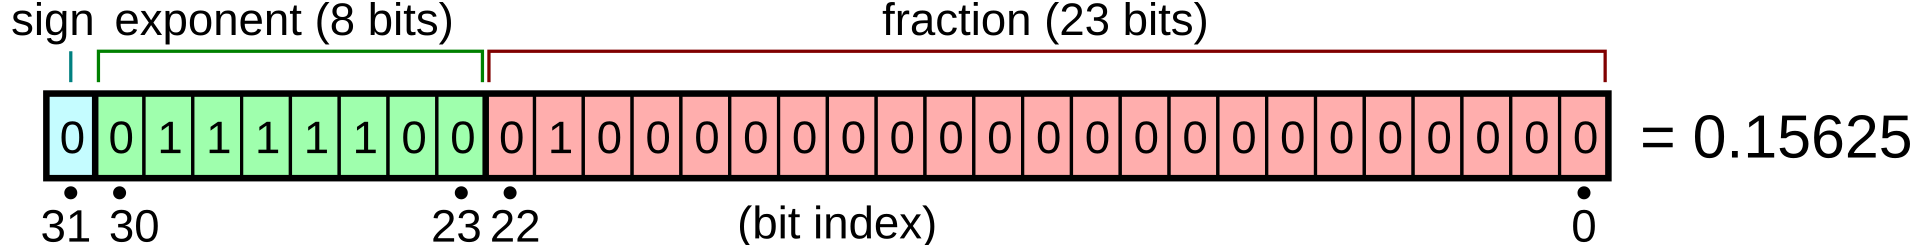
\includegraphics[width=.8\textwidth]{figures/floating-point.png}
    \caption{32-bit floating-point illustration.}
    \label{fig:floating-point}
\end{figure}

\begin{bclogo}[couleur = gray!20, arrondi = 0.2, logo=\bcinfo]{Floating point unit (FPU)}
Many processors are equipped with hardware accelerators dedicated to performing floating-points operations, named floating point units (FPU). Otherwise, the specific bitwise manipulations must be executed in software and require multiple CPU cycles for one basic operation. Check out our MCU's datasheet to find out if it is equipped with a FPU.
\end{bclogo}

\paragraph{Fixed-point} Fixed-points represents fractional numbers by splitting the bits in $i$ integer bits and $f$ fractional bits. The first integer bit may be negative if using \textit{signed fixed-point} \texttt{qi.f} or positive if using \textit{unsigned fixed-point} \texttt{uqi.f}. \autoref{fig:fixed-point} illustrates an example of signed fixed-point with $i = 4$ and $f = 4$. We often use \texttt{q1.f} (e.g. \texttt{q1.15}, shortened \texttt{q15}) such that the range is $[-1;1[$. Unlike floating-points, basic operations on fixed-points require the same bitwise manipulations as on integers, which makes them very efficient.

Keep in mind that the fixed-point representation is purely an interpretation of the bits significance. The CPU does not make any difference between integers and fixed-points. You can see in the code that the type \texttt{q15\_t} is just an alias for \texttt{int16\_t}.

\begin{figure}[H]
    \centering
    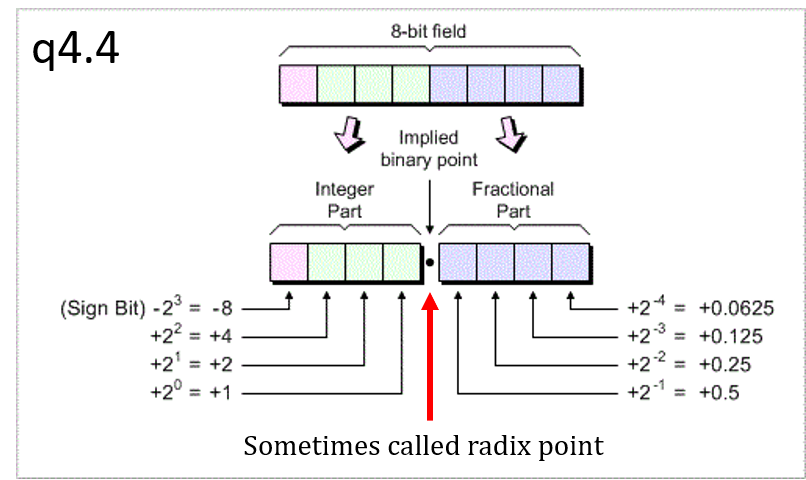
\includegraphics[width=.6\textwidth]{figures/fixed-point.png}
    \caption{8-bit fixed-point illustration.}
    \label{fig:fixed-point}
\end{figure}

\begin{bclogo}[couleur = gray!20, arrondi = 0.2, logo=\bcinfo]{Rescaling fixed-points}
By moving the radix point position using bit shifts, for example from a \texttt{q1.7} to a \texttt{q4.4} by applying $\gg3$, you change the representation without changing the value, which is called \textbf{rescaling}. This provides a tradeoff between range and resolution as you trade integer bits for fractional bits. \texttt{q1.7} has a range of $[-1;1[$ and a resolution of $2^{-7} = 0.0078125$ while \texttt{q4.4} is between $[-8;8[$ with a resolution of $2^{-4} = 0.0625$.

Rescaling fixed-points is essential when performing operations such as additions or multiplications because we want to have the best resolution possible while preventing \textbf{overflows}.
\end{bclogo}

\begin{bclogo}[couleur = gray!20, arrondi = 0.2, logo=\bcquestion]{Data representation tradeoff}
What are the pros and cons of using fixed-points rather than floating-points ? Why did we choose to use fixed-points in this project ? 
\end{bclogo}

\section{Processing the samples to a mel-vector}

\subsection{Understanding the provided code}

Open \texttt{computation.c} and read the file. It contains the implementation of \texttt{melvec\_compute()} that computes a mel-vector based on the acquired raw audio samples. Most computing functions we use are implemented in the CMSIS-DSP library and their name begins by \texttt{arm\_}.

\begin{bclogo}[couleur = gray!20, arrondi = 0.2, logo=\bcquestion]{Mel-vector computation sequence}
Draw a flow chart of the computation sequence : what operations are performed to compute a mel-vector based on raw audio samples ? Compare it with what was done in Python to compute mel-vectors from sound clips. What are the differences and similarities ?
\end{bclogo}

\begin{bclogo}[couleur = gray!20, arrondi = 0.2, logo=\bcinfo]{The CMSIS-DSP software package}
"CMSIS-DSP is an optimized compute library for embedded systems (DSP is in the name for legacy reasons)."\footnote{\url{https://github.com/ARM-software/CMSIS-DSP}} The library is included in \textbf{Drivers/CMSIS-DSP}, you can thus use any of the computation functions in the project. Check out the online documentation in \url{https://arm-software.github.io/CMSIS-DSP/v1.18.0/index.html}. For example, you can find the FFT function \texttt{arm\_fft\_q15()} in \textbf{Transform functions} $\rightarrow$ \textbf{Real FFT Functions} $\rightarrow$ \textbf{Real FFT Q15 Functions}.
\end{bclogo}

\begin{bclogo}[couleur = gray!20, arrondi = 0.2, logo=\bcinfo]{Single instruction, multiple data (SIMD)}
One key optimisation implemented in the CMSIS-DSP library is SIMD, which is the ability to process data in parallel in the CPU. For example, our MCU has a 32-bit architecture, meaning all data paths are 32-bit wide. 16-bit variables can be stacked by pairs and processed together, doubling the throughput when applying the same instruction on an array of data.
\end{bclogo}

\begin{bclogo}[couleur = gray!20, arrondi = 0.2, logo=\bcinfo]{Naive implementation}
The implementation we provide you is easily readable and undestandable, but also intentionally sub-optimal. Keep in mind that in the future you can rethink part or the whole implementation if you find better ways to implement the computation function.
\end{bclogo}

\begin{bclogo}[couleur = gray!20, arrondi = 0.2, logo=\bcinfo]{Data type and typecast}
In step $3.2$ of \texttt{computation.c}, you will observe this line of code:
\begin{lstlisting}
buf[i] = (q15_t) (((q31_t) buf_fft[i] << 15) / ((q31_t) vmax));
\end{lstlisting}
In this line, the (q15$\_$t) and two (q31$\_$t) are called \textbf{typecasts}. Typecasting consists in telling your compiler the format you wish the following variable to be stored in. Here, buf$\_$fft[i] is in q15$\_$t format, and the $\ll 15$ shifts all its bits to the left $15$ times. The casting is necessary to get a temporary q31$\_$t variable and avoid overflowing your q15$\_t$ one.
\end{bclogo}

\begin{bclogo}[couleur = gray!20, arrondi = 0.2, logo=\bcinfo]{Hardcoded data tables}
The content of \texttt{computation$\_$tables.h} has been hard-coded using the files in \textbf{classification/} \textbf{Python2C$\_$conversion}. These notebooks could be useful for you during the second semester if you want to modify the feature vector parameters. This is optional, but you can already take a look at how this is done.
\end{bclogo}

\subsection{Implementing the mel-vector computation}

% steps

% - acquisition.c : change buffer size to 512 (2 places)

% - dma callback :
%     acquisition_stop();
%     samples_buf_to_process = samples_single_buf;
%     is_processing = 1;

% - main loop : 

%         if (is_processing) {
%             melvec_compute((q15_t *)samples_buf_to_process, mel_vectors[0]);
%             print_melvectors(mel_vectors, 1);
%             is_processing = 0;
%         }


\begin{bclogo}[couleur = gray!20, arrondi = 0.2, logo=\bcattention]{Data races and volatile variables in C}
Your state variable will be a global variable, such that it can be modified in the main function and in the interrupt handler.
The main function and the interrupt handler are concurrent: they are not part of the same ``execution flow'', similarly to threads that run under an OS.
With all concurrent programming, you have to be careful the access to variables that are shared (i.e., read or written from more than one execution flow).
If at least one of the execution flow writes to a variable (concurrent reads are always ok!), the result of the execution might be non-deterministic (e.g., depend on the exact way the execution flows are interleaved), which is called a data race.
For instance, if you increment a variable (which makes 3 instructions: load, add and store) both from \texttt{main()} and from an interrupt handler, you have a data race if you take no extra precaution: if the \texttt{main()} is interrupted just after the load, the variable gets incremented by only 1 instead of 2.
In order to avoid data races, all concurrent read and writes should be either atomic (roughly, a single load/store) or synchronized (through locks, etc.).

This is further complicated by the semantics of the C programming language: it is such that the compiler can (almost) assume that there is no concurrent execution.
Therefore, if a program does not read a variable from the \texttt{main()} execution flow, it may ``optimize'' your \texttt{main()} by discarding writes to this variable, as they are ``useless''.

As a result, whenever a variable is \textbf{shared} (i.e., accessed by multiple execution flows), or represents a \textbf{memory-mapped control register}, you have to make it \textbf{volatile}. This is done by putting the qualifier \texttt{volatile} before the type in the declaration of the variable.

\textit{This was only a very limited introduction! To go further: \url{https://blog.regehr.org/archives/28}. You may also search the keywords: C memory model; atomic memory access ordering; memory barrier.}
\end{bclogo}




\begin{bclogo}[couleur = gray!20, arrondi = 0.2, logo=\bcinfo]{Interrupt callback good practice}
Be careful not to lock-up your processor: if you have a long-running interrupt handler, the MCU might not be able to respond to other events that happen.
The two common solutions are to delegate the long processing to the \texttt{main()} (and communicate that the processing should be performed by setting a state variable in the interrupt handler), or to configure the priority of the long-running interrupt such that it can be interrupted by other, higher priority, interrupts. Be careful as usually, the highest priority has the lowest value i.e. 0 being the highest priority as shown in \autoref{fig:nvic_params}.
\end{bclogo}



\section{Double-buffering technique}

